% Created by tikzDevice version 0.10.1 on 2016-06-29 16:04:46
% !TEX encoding = UTF-8 Unicode
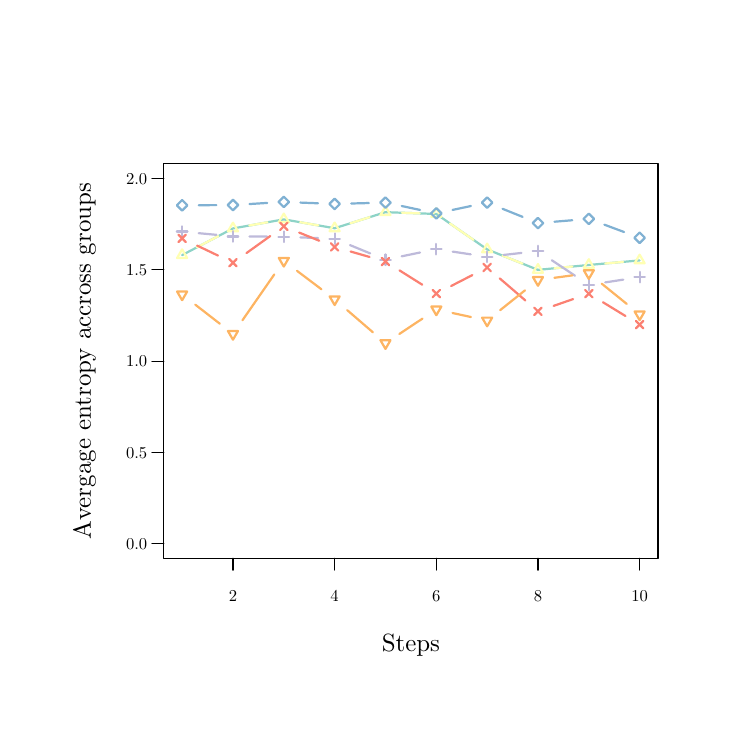
\begin{tikzpicture}[x=1pt,y=1pt]
\definecolor{fillColor}{RGB}{255,255,255}
\path[use as bounding box,fill=fillColor,fill opacity=0.00] (0,0) rectangle (252.94,252.94);
\begin{scope}
\path[clip] ( 49.20, 61.20) rectangle (227.75,203.75);
\definecolor{drawColor}{RGB}{141,211,199}

\path[draw=drawColor,line width= 0.8pt,line join=round,line cap=round] ( 55.81,170.76) --
	( 74.18,180.39) --
	( 92.55,183.67) --
	(110.92,180.46) --
	(129.29,186.27) --
	(147.66,185.62) --
	(166.03,172.82) --
	(184.39,165.42) --
	(202.76,167.19) --
	(221.13,168.84);
\end{scope}
\begin{scope}
\path[clip] (  0.00,  0.00) rectangle (252.94,252.94);
\definecolor{drawColor}{RGB}{0,0,0}

\path[draw=drawColor,line width= 0.4pt,line join=round,line cap=round] ( 74.18, 61.20) -- (221.13, 61.20);

\path[draw=drawColor,line width= 0.4pt,line join=round,line cap=round] ( 74.18, 61.20) -- ( 74.18, 56.92);

\path[draw=drawColor,line width= 0.4pt,line join=round,line cap=round] (110.92, 61.20) -- (110.92, 56.92);

\path[draw=drawColor,line width= 0.4pt,line join=round,line cap=round] (147.66, 61.20) -- (147.66, 56.92);

\path[draw=drawColor,line width= 0.4pt,line join=round,line cap=round] (184.39, 61.20) -- (184.39, 56.92);

\path[draw=drawColor,line width= 0.4pt,line join=round,line cap=round] (221.13, 61.20) -- (221.13, 56.92);

\node[text=drawColor,anchor=base,inner sep=0pt, outer sep=0pt, scale=  0.60] at ( 74.18, 45.60) {2};

\node[text=drawColor,anchor=base,inner sep=0pt, outer sep=0pt, scale=  0.60] at (110.92, 45.60) {4};

\node[text=drawColor,anchor=base,inner sep=0pt, outer sep=0pt, scale=  0.60] at (147.66, 45.60) {6};

\node[text=drawColor,anchor=base,inner sep=0pt, outer sep=0pt, scale=  0.60] at (184.39, 45.60) {8};

\node[text=drawColor,anchor=base,inner sep=0pt, outer sep=0pt, scale=  0.60] at (221.13, 45.60) {10};

\path[draw=drawColor,line width= 0.4pt,line join=round,line cap=round] ( 49.20, 66.48) -- ( 49.20,198.47);

\path[draw=drawColor,line width= 0.4pt,line join=round,line cap=round] ( 49.20, 66.48) -- ( 44.92, 66.48);

\path[draw=drawColor,line width= 0.4pt,line join=round,line cap=round] ( 49.20, 99.48) -- ( 44.92, 99.48);

\path[draw=drawColor,line width= 0.4pt,line join=round,line cap=round] ( 49.20,132.47) -- ( 44.92,132.47);

\path[draw=drawColor,line width= 0.4pt,line join=round,line cap=round] ( 49.20,165.47) -- ( 44.92,165.47);

\path[draw=drawColor,line width= 0.4pt,line join=round,line cap=round] ( 49.20,198.47) -- ( 44.92,198.47);

\node[text=drawColor,anchor=base east,inner sep=0pt, outer sep=0pt, scale=  0.60] at ( 43.20, 64.41) {0.0};

\node[text=drawColor,anchor=base east,inner sep=0pt, outer sep=0pt, scale=  0.60] at ( 43.20, 97.41) {0.5};

\node[text=drawColor,anchor=base east,inner sep=0pt, outer sep=0pt, scale=  0.60] at ( 43.20,130.41) {1.0};

\node[text=drawColor,anchor=base east,inner sep=0pt, outer sep=0pt, scale=  0.60] at ( 43.20,163.40) {1.5};

\node[text=drawColor,anchor=base east,inner sep=0pt, outer sep=0pt, scale=  0.60] at ( 43.20,196.40) {2.0};

\path[draw=drawColor,line width= 0.4pt,line join=round,line cap=round] ( 49.20, 61.20) --
	(227.75, 61.20) --
	(227.75,203.75) --
	( 49.20,203.75) --
	( 49.20, 61.20);
\end{scope}
\begin{scope}
\path[clip] (  0.00,  0.00) rectangle (252.94,252.94);
\definecolor{drawColor}{RGB}{0,0,0}

\node[text=drawColor,anchor=base,inner sep=0pt, outer sep=0pt, scale=  0.90] at (138.47, 27.60) {Steps};

\node[text=drawColor,rotate= 90.00,anchor=base,inner sep=0pt, outer sep=0pt, scale=  0.90] at ( 22.80,132.47) {Avergage entropy accross groups};
\end{scope}
\begin{scope}
\path[clip] ( 49.20, 61.20) rectangle (227.75,203.75);
\definecolor{drawColor}{RGB}{255,255,179}

\path[draw=drawColor,line width= 0.8pt,line join=round,line cap=round] ( 61.13,173.55) -- ( 68.87,177.61);

\path[draw=drawColor,line width= 0.8pt,line join=round,line cap=round] ( 80.09,181.45) -- ( 86.64,182.62);

\path[draw=drawColor,line width= 0.8pt,line join=round,line cap=round] ( 98.46,182.64) -- (105.01,181.49);

\path[draw=drawColor,line width= 0.8pt,line join=round,line cap=round] (116.64,182.27) -- (123.57,184.46);

\path[draw=drawColor,line width= 0.8pt,line join=round,line cap=round] (135.28,186.06) -- (141.66,185.83);

\path[draw=drawColor,line width= 0.8pt,line join=round,line cap=round] (152.58,182.19) -- (161.10,176.25);

\path[draw=drawColor,line width= 0.8pt,line join=round,line cap=round] (171.59,170.58) -- (178.83,167.66);

\path[draw=drawColor,line width= 0.8pt,line join=round,line cap=round] (190.37,166.00) -- (196.79,166.62);

\path[draw=drawColor,line width= 0.8pt,line join=round,line cap=round] (208.74,167.73) -- (215.16,168.30);

\path[draw=drawColor,line width= 0.8pt,line join=round,line cap=round] ( 55.81,172.86) --
	( 57.63,169.71) --
	( 53.99,169.71) --
	( 55.81,172.86);

\path[draw=drawColor,line width= 0.8pt,line join=round,line cap=round] ( 74.18,182.49) --
	( 76.00,179.34) --
	( 72.36,179.34) --
	( 74.18,182.49);

\path[draw=drawColor,line width= 0.8pt,line join=round,line cap=round] ( 92.55,185.77) --
	( 94.37,182.62) --
	( 90.73,182.62) --
	( 92.55,185.77);

\path[draw=drawColor,line width= 0.8pt,line join=round,line cap=round] (110.92,182.55) --
	(112.74,179.41) --
	(109.10,179.41) --
	(110.92,182.55);

\path[draw=drawColor,line width= 0.8pt,line join=round,line cap=round] (129.29,188.37) --
	(131.11,185.22) --
	(127.47,185.22) --
	(129.29,188.37);

\path[draw=drawColor,line width= 0.8pt,line join=round,line cap=round] (147.66,187.72) --
	(149.48,184.57) --
	(145.84,184.57) --
	(147.66,187.72);

\path[draw=drawColor,line width= 0.8pt,line join=round,line cap=round] (166.03,174.92) --
	(167.84,171.77) --
	(164.21,171.77) --
	(166.03,174.92);

\path[draw=drawColor,line width= 0.8pt,line join=round,line cap=round] (184.39,167.52) --
	(186.21,164.37) --
	(182.58,164.37) --
	(184.39,167.52);

\path[draw=drawColor,line width= 0.8pt,line join=round,line cap=round] (202.76,169.29) --
	(204.58,166.14) --
	(200.95,166.14) --
	(202.76,169.29);

\path[draw=drawColor,line width= 0.8pt,line join=round,line cap=round] (221.13,170.94) --
	(222.95,167.79) --
	(219.31,167.79) --
	(221.13,170.94);
\definecolor{drawColor}{RGB}{190,186,218}

\path[draw=drawColor,line width= 0.8pt,line join=round,line cap=round] ( 61.79,178.68) -- ( 68.21,178.08);

\path[draw=drawColor,line width= 0.8pt,line join=round,line cap=round] ( 80.18,177.48) -- ( 86.55,177.44);

\path[draw=drawColor,line width= 0.8pt,line join=round,line cap=round] ( 98.55,177.16) -- (104.92,176.90);

\path[draw=drawColor,line width= 0.8pt,line join=round,line cap=round] (116.47,174.37) -- (123.74,171.38);

\path[draw=drawColor,line width= 0.8pt,line join=round,line cap=round] (135.16,170.32) -- (141.78,171.69);

\path[draw=drawColor,line width= 0.8pt,line join=round,line cap=round] (153.59,172.01) -- (160.09,171.03);

\path[draw=drawColor,line width= 0.8pt,line join=round,line cap=round] (171.99,170.81) -- (178.43,171.54);

\path[draw=drawColor,line width= 0.8pt,line join=round,line cap=round] (189.39,168.89) -- (197.77,163.31);

\path[draw=drawColor,line width= 0.8pt,line join=round,line cap=round] (208.69,160.89) -- (215.20,161.89);

\path[draw=drawColor,line width= 0.8pt,line join=round,line cap=round] ( 53.90,179.25) -- ( 57.72,179.25);

\path[draw=drawColor,line width= 0.8pt,line join=round,line cap=round] ( 55.81,177.34) -- ( 55.81,181.16);

\path[draw=drawColor,line width= 0.8pt,line join=round,line cap=round] ( 72.27,177.51) -- ( 76.09,177.51);

\path[draw=drawColor,line width= 0.8pt,line join=round,line cap=round] ( 74.18,175.60) -- ( 74.18,179.42);

\path[draw=drawColor,line width= 0.8pt,line join=round,line cap=round] ( 90.64,177.40) -- ( 94.46,177.40);

\path[draw=drawColor,line width= 0.8pt,line join=round,line cap=round] ( 92.55,175.49) -- ( 92.55,179.31);

\path[draw=drawColor,line width= 0.8pt,line join=round,line cap=round] (109.01,176.65) -- (112.83,176.65);

\path[draw=drawColor,line width= 0.8pt,line join=round,line cap=round] (110.92,174.74) -- (110.92,178.56);

\path[draw=drawColor,line width= 0.8pt,line join=round,line cap=round] (127.38,169.10) -- (131.20,169.10);

\path[draw=drawColor,line width= 0.8pt,line join=round,line cap=round] (129.29,167.19) -- (129.29,171.01);

\path[draw=drawColor,line width= 0.8pt,line join=round,line cap=round] (145.75,172.91) -- (149.57,172.91);

\path[draw=drawColor,line width= 0.8pt,line join=round,line cap=round] (147.66,171.00) -- (147.66,174.82);

\path[draw=drawColor,line width= 0.8pt,line join=round,line cap=round] (164.12,170.13) -- (167.93,170.13);

\path[draw=drawColor,line width= 0.8pt,line join=round,line cap=round] (166.03,168.22) -- (166.03,172.04);

\path[draw=drawColor,line width= 0.8pt,line join=round,line cap=round] (182.49,172.22) -- (186.30,172.22);

\path[draw=drawColor,line width= 0.8pt,line join=round,line cap=round] (184.39,170.31) -- (184.39,174.12);

\path[draw=drawColor,line width= 0.8pt,line join=round,line cap=round] (200.85,159.98) -- (204.67,159.98);

\path[draw=drawColor,line width= 0.8pt,line join=round,line cap=round] (202.76,158.07) -- (202.76,161.89);

\path[draw=drawColor,line width= 0.8pt,line join=round,line cap=round] (219.22,162.80) -- (223.04,162.80);

\path[draw=drawColor,line width= 0.8pt,line join=round,line cap=round] (221.13,160.89) -- (221.13,164.71);
\definecolor{drawColor}{RGB}{251,128,114}

\path[draw=drawColor,line width= 0.8pt,line join=round,line cap=round] ( 61.23,174.20) -- ( 68.77,170.59);

\path[draw=drawColor,line width= 0.8pt,line join=round,line cap=round] ( 79.06,171.49) -- ( 87.67,177.65);

\path[draw=drawColor,line width= 0.8pt,line join=round,line cap=round] ( 98.11,178.89) -- (105.36,175.95);

\path[draw=drawColor,line width= 0.8pt,line join=round,line cap=round] (116.69,172.05) -- (123.52,170.09);

\path[draw=drawColor,line width= 0.8pt,line join=round,line cap=round] (134.36,165.23) -- (142.58,160.06);

\path[draw=drawColor,line width= 0.8pt,line join=round,line cap=round] (153.00,159.59) -- (160.69,163.53);

\path[draw=drawColor,line width= 0.8pt,line join=round,line cap=round] (170.57,162.35) -- (179.85,154.36);

\path[draw=drawColor,line width= 0.8pt,line join=round,line cap=round] (190.06,152.41) -- (197.10,154.86);

\path[draw=drawColor,line width= 0.8pt,line join=round,line cap=round] (207.89,153.71) -- (216.01,148.75);

\path[draw=drawColor,line width= 0.8pt,line join=round,line cap=round] ( 54.46,175.43) -- ( 57.16,178.13);

\path[draw=drawColor,line width= 0.8pt,line join=round,line cap=round] ( 54.46,178.13) -- ( 57.16,175.43);

\path[draw=drawColor,line width= 0.8pt,line join=round,line cap=round] ( 72.83,166.65) -- ( 75.53,169.35);

\path[draw=drawColor,line width= 0.8pt,line join=round,line cap=round] ( 72.83,169.35) -- ( 75.53,166.65);

\path[draw=drawColor,line width= 0.8pt,line join=round,line cap=round] ( 91.20,179.79) -- ( 93.90,182.49);

\path[draw=drawColor,line width= 0.8pt,line join=round,line cap=round] ( 91.20,182.49) -- ( 93.90,179.79);

\path[draw=drawColor,line width= 0.8pt,line join=round,line cap=round] (109.57,172.35) -- (112.27,175.05);

\path[draw=drawColor,line width= 0.8pt,line join=round,line cap=round] (109.57,175.05) -- (112.27,172.35);

\path[draw=drawColor,line width= 0.8pt,line join=round,line cap=round] (127.94,167.08) -- (130.64,169.78);

\path[draw=drawColor,line width= 0.8pt,line join=round,line cap=round] (127.94,169.78) -- (130.64,167.08);

\path[draw=drawColor,line width= 0.8pt,line join=round,line cap=round] (146.31,155.51) -- (149.01,158.21);

\path[draw=drawColor,line width= 0.8pt,line join=round,line cap=round] (146.31,158.21) -- (149.01,155.51);

\path[draw=drawColor,line width= 0.8pt,line join=round,line cap=round] (164.68,164.92) -- (167.38,167.62);

\path[draw=drawColor,line width= 0.8pt,line join=round,line cap=round] (164.68,167.62) -- (167.38,164.92);

\path[draw=drawColor,line width= 0.8pt,line join=round,line cap=round] (183.04,149.09) -- (185.74,151.79);

\path[draw=drawColor,line width= 0.8pt,line join=round,line cap=round] (183.04,151.79) -- (185.74,149.09);

\path[draw=drawColor,line width= 0.8pt,line join=round,line cap=round] (201.41,155.48) -- (204.11,158.18);

\path[draw=drawColor,line width= 0.8pt,line join=round,line cap=round] (201.41,158.18) -- (204.11,155.48);

\path[draw=drawColor,line width= 0.8pt,line join=round,line cap=round] (219.78,144.28) -- (222.48,146.98);

\path[draw=drawColor,line width= 0.8pt,line join=round,line cap=round] (219.78,146.98) -- (222.48,144.28);
\definecolor{drawColor}{RGB}{128,177,211}

\path[draw=drawColor,line width= 0.8pt,line join=round,line cap=round] ( 61.81,188.79) -- ( 68.18,188.82);

\path[draw=drawColor,line width= 0.8pt,line join=round,line cap=round] ( 80.17,189.21) -- ( 86.56,189.61);

\path[draw=drawColor,line width= 0.8pt,line join=round,line cap=round] ( 98.55,189.73) -- (104.92,189.48);

\path[draw=drawColor,line width= 0.8pt,line join=round,line cap=round] (116.92,189.40) -- (123.29,189.57);

\path[draw=drawColor,line width= 0.8pt,line join=round,line cap=round] (135.16,188.49) -- (141.79,187.08);

\path[draw=drawColor,line width= 0.8pt,line join=round,line cap=round] (153.53,187.08) -- (160.16,188.49);

\path[draw=drawColor,line width= 0.8pt,line join=round,line cap=round] (171.59,187.49) -- (178.83,184.57);

\path[draw=drawColor,line width= 0.8pt,line join=round,line cap=round] (190.37,182.82) -- (196.78,183.35);

\path[draw=drawColor,line width= 0.8pt,line join=round,line cap=round] (208.39,181.75) -- (215.51,179.10);

\path[draw=drawColor,line width= 0.8pt,line join=round,line cap=round] ( 53.90,188.76) --
	( 55.81,190.66) --
	( 57.72,188.76) --
	( 55.81,186.85) --
	( 53.90,188.76);

\path[draw=drawColor,line width= 0.8pt,line join=round,line cap=round] ( 72.27,188.85) --
	( 74.18,190.76) --
	( 76.09,188.85) --
	( 74.18,186.94) --
	( 72.27,188.85);

\path[draw=drawColor,line width= 0.8pt,line join=round,line cap=round] ( 90.64,189.97) --
	( 92.55,191.88) --
	( 94.46,189.97) --
	( 92.55,188.07) --
	( 90.64,189.97);

\path[draw=drawColor,line width= 0.8pt,line join=round,line cap=round] (109.01,189.24) --
	(110.92,191.15) --
	(112.83,189.24) --
	(110.92,187.33) --
	(109.01,189.24);

\path[draw=drawColor,line width= 0.8pt,line join=round,line cap=round] (127.38,189.73) --
	(129.29,191.64) --
	(131.20,189.73) --
	(129.29,187.83) --
	(127.38,189.73);

\path[draw=drawColor,line width= 0.8pt,line join=round,line cap=round] (145.75,185.83) --
	(147.66,187.74) --
	(149.57,185.83) --
	(147.66,183.92) --
	(145.75,185.83);

\path[draw=drawColor,line width= 0.8pt,line join=round,line cap=round] (164.12,189.73) --
	(166.03,191.64) --
	(167.93,189.73) --
	(166.03,187.83) --
	(164.12,189.73);

\path[draw=drawColor,line width= 0.8pt,line join=round,line cap=round] (182.49,182.33) --
	(184.39,184.24) --
	(186.30,182.33) --
	(184.39,180.42) --
	(182.49,182.33);

\path[draw=drawColor,line width= 0.8pt,line join=round,line cap=round] (200.85,183.85) --
	(202.76,185.76) --
	(204.67,183.85) --
	(202.76,181.94) --
	(200.85,183.85);

\path[draw=drawColor,line width= 0.8pt,line join=round,line cap=round] (219.22,177.01) --
	(221.13,178.92) --
	(223.04,177.01) --
	(221.13,175.10) --
	(219.22,177.01);
\definecolor{drawColor}{RGB}{253,180,98}

\path[draw=drawColor,line width= 0.8pt,line join=round,line cap=round] ( 60.55,152.86) -- ( 69.44,145.96);

\path[draw=drawColor,line width= 0.8pt,line join=round,line cap=round] ( 77.61,147.21) -- ( 89.12,163.77);

\path[draw=drawColor,line width= 0.8pt,line join=round,line cap=round] ( 97.33,165.07) -- (106.14,158.41);

\path[draw=drawColor,line width= 0.8pt,line join=round,line cap=round] (115.46,150.87) -- (124.74,142.87);

\path[draw=drawColor,line width= 0.8pt,line join=round,line cap=round] (134.29,142.26) -- (142.65,147.80);

\path[draw=drawColor,line width= 0.8pt,line join=round,line cap=round] (153.52,149.83) -- (160.16,148.39);

\path[draw=drawColor,line width= 0.8pt,line join=round,line cap=round] (170.72,150.85) -- (179.70,158.02);

\path[draw=drawColor,line width= 0.8pt,line join=round,line cap=round] (190.34,162.56) -- (196.82,163.43);

\path[draw=drawColor,line width= 0.8pt,line join=round,line cap=round] (207.42,160.45) -- (216.47,153.12);

\path[draw=drawColor,line width= 0.8pt,line join=round,line cap=round] ( 55.81,154.44) --
	( 57.63,157.59) --
	( 53.99,157.59) --
	( 55.81,154.44);

\path[draw=drawColor,line width= 0.8pt,line join=round,line cap=round] ( 74.18,140.18) --
	( 76.00,143.33) --
	( 72.36,143.33) --
	( 74.18,140.18);

\path[draw=drawColor,line width= 0.8pt,line join=round,line cap=round] ( 92.55,166.60) --
	( 94.37,169.74) --
	( 90.73,169.74) --
	( 92.55,166.60);

\path[draw=drawColor,line width= 0.8pt,line join=round,line cap=round] (110.92,152.69) --
	(112.74,155.83) --
	(109.10,155.83) --
	(110.92,152.69);

\path[draw=drawColor,line width= 0.8pt,line join=round,line cap=round] (129.29,136.85) --
	(131.11,140.00) --
	(127.47,140.00) --
	(129.29,136.85);

\path[draw=drawColor,line width= 0.8pt,line join=round,line cap=round] (147.66,149.01) --
	(149.48,152.16) --
	(145.84,152.16) --
	(147.66,149.01);

\path[draw=drawColor,line width= 0.8pt,line join=round,line cap=round] (166.03,145.01) --
	(167.84,148.16) --
	(164.21,148.16) --
	(166.03,145.01);

\path[draw=drawColor,line width= 0.8pt,line join=round,line cap=round] (184.39,159.66) --
	(186.21,162.81) --
	(182.58,162.81) --
	(184.39,159.66);

\path[draw=drawColor,line width= 0.8pt,line join=round,line cap=round] (202.76,162.13) --
	(204.58,165.28) --
	(200.95,165.28) --
	(202.76,162.13);

\path[draw=drawColor,line width= 0.8pt,line join=round,line cap=round] (221.13,147.24) --
	(222.95,150.39) --
	(219.31,150.39) --
	(221.13,147.24);
\end{scope}
\end{tikzpicture}
